\documentclass[a4paper, 12pt]{report}
\usepackage[ngerman]{babel}
\usepackage{amssymb}
\usepackage{tabularx}
\usepackage[utf8]{inputenc}
\usepackage{amsmath}
\usepackage{bbm}
\usepackage{setspace}
\usepackage{fancyvrb}
\usepackage{graphicx}
\usepackage[style=alphabetic ,backend=biber]{biblatex}
\usepackage{csquotes}
\usepackage{array}
\usepackage{geometry}
\geometry{
 a4paper,
 total={170mm,257mm},
 left=25mm,
 right=40mm,
 top=25mm,
 bottom=40mm
 }
 \setstretch{1.5}
\addbibresource{../Facharbeit/literatur.bib}
\usepackage{listings}
\usepackage{xcolor}


\definecolor{codegreen}{rgb}{0,0.6,0}
\definecolor{codegray}{rgb}{0.5,0.5,0.5}
\definecolor{codepurple}{rgb}{0.58,0,0.82}
\definecolor{backcolour}{rgb}{255,255,255}

\lstdefinestyle{codehighligthing}{
    backgroundcolor=\color{backcolour},
    commentstyle=\color{codegreen},
    keywordstyle=\color{magenta},
    numberstyle=\tiny\color{codegray},
    stringstyle=\color{codepurple},
    basicstyle=\ttfamily\tiny,
    breakatwhitespace=false,
    breaklines=true,
    captionpos=b,
    keepspaces=true,
    numbers=left,
    numbersep=5pt,
    showspaces=false,
    showstringspaces=false,
    showtabs=false,
    tabsize=2,
}
\lstset{style=codehighligthing}


\title{\LARGE Facharbeit im Grundkurs Informatik  \vspace*{0.5cm} \\
  \Huge Implementation des Gauß-Algorithmus \vspace*{0.5cm} \\
  \LARGE Georg-Büchner-Gymnasium}
\LARGE \author{Joel Mantik
\vspace*{0.5cm} \\ Pablo Sonnauer}
\LARGE \date{März 2023}
\begin{document}
\maketitle
\begin{sloppypar}
\tableofcontents

\chapter{Einleitung}
\begin{quote}
    "The simplest model in applied mathematics is a system of linear equations. It is also by far the most important."
    \newline GILBERT STRANG
\end{quote}
Der Gauß-Algorithmus ist eins der wichtigsten Lösungsverfahren zum Lösen linearer Gleichungssysteme.
Er spielt eine tragende Rolle in vielen Bereichen der Mathematik und ist dennoch  recht unkompliziert.
    Aufgrund der Wichtigkeit, habe ich dazu entschieden, den Algorithmus in dieser
Facharbeit zu implementieren,
zu analysieren, und Anwendungsmöglichkeiten aufzuzeigen.

{\let\clearpage\relax \chapter{Theoretische Grundlagen}}

Der Gauß-Algorithmus ist ein Algorithmus, welcher beim Lösen von linearen Gleichungssystemen zum Einsatz kommt.
Im folgenden Kapitel wird die mathematische
Theorie erläutert und die Definitionen genannt, welche die Grundlage für die spätere Implementierung sind.

{\let\clearpage\relax \section{Lineare Gleichungssysteme}}
Ein lineares Gleichungssystem ist eine Sammlung von Gleichungen, in denen jede Unbekannte mit höchstens
dem ersten Grad vorkommt.
Es kann in der Form $ A_x = b $ geschrieben werden, wobei $A$ eine $ m x n $ Matrix ist,
$x$ ein n-dimensionaler Vektor von Unbekannten
und b ein $m$-dimensionaler Vektor von Konstanten ist.
Ein allgemeines lineares Gleichungssystem lässt sich wie folgt definieren.: \cite{1}
\begin{align}
\label{eq:linGle}
    a_{11}x_{1}+ a_{12}x_{2}+\hdots+ a_{1n}x_{n} &=& b_1 \nonumber \\
    a_{21}x_{1}+ a_{22}x_{2}+\hdots+ a_{2n}x_{n} &=& b_2 \nonumber\\
                                                 &\vdots&  \nonumber \\
    a_{m1}x_{1}+ a_{m2}x_2+\hdots+a_{mn}x_{n} &=& b_{m}
\end{align}
Das Ziel eines solchen linearen Gleichungssystems ist es, eine Lösung für $x$ zu finden, die alle Gleichungen erfüllt.
Hierbei gibt es drei Arten von Lösungen:
\begin{enumerate}
    \item Das Gleichungssystem hat genau \textit{eine} Lösung;
        es gibt genau eine Lösung, welche alle Gleichungen im System
        erfüllt. Die Lösungsmenge ist z. B. : $\mathbb{L} = \{ (x,y,z)| (1,2,3)\} $.
    \item Das Gleichungssystem hat \textit{keine} Lösung, wenn es keine Lösung gibt,
        die alle Gleichungen erfüllt. Die Lösungsmenge ist eine leere Menge: $ \mathbb{L}= \emptyset$.
    \item Das Gleichungssystem hat \textit{unendlich viele} Lösungen, wenn es mehrere Lösungen gibt
        die alle Gleichungen im System erfüllen.
        Hierbei sind die verschiedenen Variablen voneinander abhängig.
        Die Lösungsmenge sieht beispielsweise wie folgt aus:
        \newline $ \mathbb{L} = \{(x, y, z)| (x = ay + z, y\in \mathbb{R}, z \in \mathbb{R}) \} $.
\end{enumerate}


\section{Gaußsches Eliminationsverfahren} \label{2.2}
Gegeben sei das Allgemeine Lineare Gleichungssystem \ref{eq:linGle}.
Gesucht ist nun die Menge der $ (x_1, \hdots ,x_n ) \in \mathbb{R}^n $, die alle Gleichungen erfüllen.
Dies erreicht man, indem man folgendermaßen vorgeht.:
\begin{enumerate}
    \item Die erweiterte Koeffizientenmatrix $ (A, b) $ aufschreiben. \cite{2}:
        \begin{equation}
            (A, b):=
            \begin{pmatrix}
                a_{11} & \hdots &  a_{1n} &  b_1  \\
                \vdots & \vdots &  \vdots & \vdots &  \\
                a_{m1} &  \hdots &  a_{mn} &  b_m \\
            \end{pmatrix}
        \end{equation}
    \item $A$ durch elementare Zeilentransformationen, also Vertauschen von Zeilen,
        Multiplikation einer Zeile mit einer Zahl $\neq 0 $ oder Addition des Vielfachen von einer Zeile zu einer
        anderen Zeile auf Zeilenstufenform bringen.
        Eine $ m x n $-Matrix A heißt in \textit{Zeilenstufenform},
        wenn sie von der folgenden Form ist: \newline \newline
        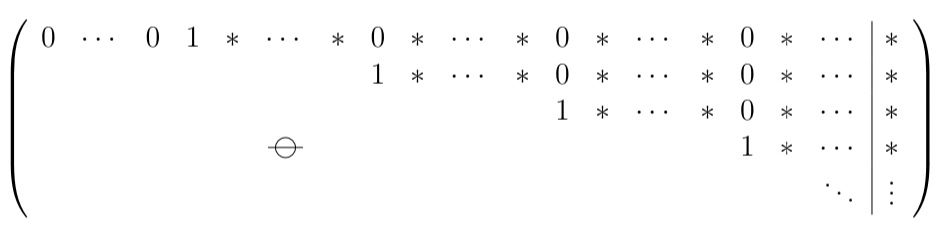
\includegraphics[width=350px]{"./Zeilenstufenform.jpeg"} \newline \newline
        Dabei steht der Stern für eine beliebige Zahl, und die freien Plätze sind alle mit Nullen besetzt.
        Der erste von Null verschiedene Eintrag in jeder Zeile ist 1. Dieser Eintrag wird das Pivot-Element der Zeile genannt.
        Das Pivot-Element der $(i + 1)$-ten Zeile steht immer rechts des Pivot-Elements der i-ten Zeile, und alle Einträge
        oberhalb eines Pivot-Elements sind gleich Null. \cite{5}
    \item Nun lassen sich durch Rücksubstitution die Werte für die Variablen ermitteln.
        Man teilt die letzte Spalte durch den Wert des Koeffizienten, so dass die Variable alleine steht.
          Der gefundene Wert wird dann in die nächst höhere Zeile eingesetzt, dann wird analog zum ersten Schritt vorgegangen.
\end{enumerate}

{\let\clearpage\relax \chapter{Erläuterung des Quellcodes}}
Für die im Folgenden dargelegte Implementation und Analyse des Algorithmus wurde die Programmiersprache "Java" verwendet.

Der grundlegende Aufbau des Programms lässt sich an folgendem Implementationsdiagramm erkennen.: \newline
\begin{center}
\footnotesize
\begin{tabularx}{0.8\textwidth} {
     | >{\raggedright\arraybackslash}X |}
    \hline
    Gauss &
    \hline
    - datei:String  & - koeff: double[][] & - solMatrix: double[][] & - zeilenElemente: String[] &
    - countSpalten: int & - countZeilen: int & - SONDERFALL: boolean &
    - NORMALFALL: boolean &
    \hline
    - main(args: String[]): void &
    - einlesen(): void &
    - ausgabe(): void &
    - gaussAlgo(): void &
    - multiplyAndAdd(lineOne: int, lineTwo: int, factor: double): void &
    - checkWievielNullZeilen(): boolean &
    -checkObNull(zeile: int): boolean &
    \hline
\end{tabularx}
\newline
\end{center}
Die Namen der Methoden wurden so gewählt, dass die Grundfunktion dieser klar sind.
In der Main Methode des Programms wird ein Parameter übernommen,
welcher die Datei mit der Koeffizientenmatrix annimmt. Außerdem werden
in dieser die Methoden \texttt{einlesen(), ausgabe() und gaussAlgo()} ausgeführt.
Die Methode \texttt{ausgabe()} gibt in der Main Methode
sowohl die Eingangsmatrix als auch die Lösungsmatrix aus. \newline
Die Methode \texttt{einlesen()} liest die Koeffizientenmatrix aus der Datei ein,
dabei wird eine Liste erstellt, in welcher alle Zeilen der eingelesenen Datei gespeichert werden.
Dann werden durch eine For-Schleife alle Leerzeichen und Kommentare entfernt. Des Weiteren werden die Kommata zu Punkten gemacht,
um das Funktionieren des Algorithmus auch auf anderen Systemen zu gewährleisten.
Weiterhin wird die Anzahl der Spalten in der Variable \texttt{countSpalten},
und die Anzahl der Zeilen in \texttt{countZeilen} gespeichert und
im Zuge dessen auch die \textit{Eingangsmatrix} \texttt{koeff[][]}und die \textit{Lösungsmatrix} \texttt{solMatrix[][]}initialisiert.
Die Methode \texttt{ausgabe()} nimmt zwei Parameter an, den zweidimensionalen Array \texttt{double mx}
und den String \texttt{matrixName}. Beide werden durch eine For-Schleife auf der Konsole ausgegeben.
Die Methode \texttt{multiplyAndAdd()}, welche die Parameter \texttt{lineOne, lineTwo (Integer)}
und den \texttt{double factor} annimmt, wird verwendet um, die Koeffizienten zu einer Null zu machen.
Dabei wird durch eine For-Schleife über die Spalten der Matrix iteriert
und dabei der Koeffizient an der Stelle von \texttt{lineTwo} und \texttt{spalten} auf den Wert Null gebracht.
Dies geschieht, indem die Matrix an der Stelle \texttt{lineOne} und \texttt{spalten} mit dem Parameter \texttt{factor} multipliziert
und zu dem zu verändernden Koeffizienten addiert.
Weiter gibt es die Methode \texttt{checkObNull()}, welche den Parameter \texttt{zeile (Integer)} annimmt
und über die Eingangsmartix iteriert und prüft ob ein Koeffizient den Wert Null hat, wenn es einen solchen Fall gibt
wird \texttt{true} zurückgegeben, andernfalls \texttt{false}.
Diese Methode wird später für die Sonderbehandlung von nicht normalen Matrizes verwendet.
Anknüpfend gibt es noch die Methode \texttt{checkWievielNullZeilen()}. Diese iteriert, ausgehend von der dritten Zeile,
über die Zeilen und prüft für jede, ob die Koeffizienten in der Zeile gleich null sind. Für jede gefundene Null-Zeile wird, ein Counter
\texttt{nullCounter} erhöht. Wenn diese Zählvariable am Ende der Iteration ungleich Null ist, wird die Konstante \texttt{SONDERFALL} zurückgegeben
und die Anzahl der Null-Zeilen auf der Konsole ausgegeben, andernfalls wird die Konstante \texttt{NORMALFALL} zurückgegeben.
Wenn die Matrix an jeder Stelle eine Null hat, wird ebenfalls interveniert und die Fehlermeldung auf der Konsole ausgegeben.
Die Methode arbeitet sehr effektiv, denn durch die Pivotisierung kann, wie bereits erwähnt, von hinten iteriert werden, denn
wenn es Null-Zeilen gibt so sind diese am Ende.

Die Methode \texttt{gaussAlgo()} ist die Methode in der eigentliche Algorithmus passiert.
Als Erstes wird die Eingangsmartix also \texttt{koeff[][]}, durch eine For-Schleife, in die Lösungsmatrix \texttt{solMatrix[][]} kopiert, damit am Ende
beide ausgegeben werden können.
Anschließend findet die Pivotisierung der Matrix statt. Dies geschieht, indem zuerst,
eine Variable \texttt{maxZeile (Integer)} erzeugt und mit der Zählvariable \texttt{zeile} initialisiert wird.
Diese wird verwendet, um die Zeile mit dem größten Koeffizienten zu finden.
In der darauf folgenden for-Schleife findet die eigentliche Pivotisierung statt.
Sie sucht in der aktuellen Spalte nach dem Element mit dem größten, absoluten Wert
und speichert diesen, wenn der größere Wert in der Zeile unter der aktuellen Zeile ist in der Variable \texttt{maxZeile}.
Anschließend folgt eine If-Bedingung: Wenn die zuvor initialisierte maxZeile ungleich dem Wert der Variable \texttt{zeile} ist,
werden die Zeilen mithilfe einer temporären Variable getauscht, sodass am Ende die
Zahl mit dem größten Koeffizienten oben steht.
Die nächste For-Schleife berechnet den Faktor \texttt{factor}, indem die Lösungsmatrix mit negativem Vorzeichen an der Stelle der Zählvariable i
und \texttt{zeile} (die Zählvariable der ersten for-Schleife), durch die Lösungsmatrix an der Stelle \texttt{zeile, zeile} geteilt wird.
Dieser Faktor wird dann an die Methode \texttt{multiplyAndAdd} zusammen mit \texttt{zeile, i} als Parameter übergeben, nachdem
die For-Schleife durchgelaufen ist, wird die hergestellte triangularisierte Matrix  ausgegeben. Anschließend prüft der Algorithmus
die triangularisierte Matrix indem durch eine If-Bedingung abgefragt wird, ob die Methode \texttt{checkWievielNullZeilen} auf
die Matrix angewendet wird, wenn sie ein Sonderfall zurückgibt, bricht der Algorithmus ab.
Der letzte Schritt, wird verwendet, um die Matrix durch Rücksubstitution zu lösen.
Eine For-Schleife läuft von der letzten Spalte bis zur ersten. Zuerst wird in dieser Schleife eine Variable \texttt{double diagonale}
erstellt, in welcher das aktuelle Diagonalelement gespeichert wird. In der nächsten Zeile iteriert eine weitere For-Schleife
über die Matrix und teilt bei jeder Iteration den Wert des aktuellen Koeffizienten durch den Wert in \texttt{diagonale}.
Dadurch entsteht die Dreiecksform, bei welcher jedes Element in dieser den Wert Eins haben soll.
Weitergehend wird der Wert des Tupels in der Variable \texttt{double result} gespeichert.
Durch eine weitere For-Schleife wird die über alle Zeilen unter der aktuellen iteriert, bei jeder Iteration wird der Wert
der rechten Zeile um das Produkt aus dem Wert von \texttt{result} und dem Wert des Elements aus der aktuellen Spalte der Zeile
subtrahiert. Als Letztes wird noch der Wert der aktuellen Zeile auf null gesetzt, damit das Gleichungssystem in der Dreiecksform
bleibt.





{\let\clearpage\relax \chapter{Abwägungen}}

\section{Vorteile des Algorithmus}
Der Gauß-Algorithmus hat klar den Vorteil das er bei Gleichungssystemen mit wenig Koeffizienten
sehr effektiv ist, d.h er kann die Lösung schnell und einfach berechnen.
Auch ist der Algorithmus in der Programmierung relativ leicht umzusetzen,
da er nach einfachen Schemata funktioniert, bei welchem wenige Schritte benötigt werden.
\section{Nachteile des Algorithmus}
Zum einen kann es durch die Verwendung vom Datentyp Double und die mehrfache Rechnung mit denselben Werten zu Rundungsfehlern kommen.
Zum anderen hat der Algorithmus bei komplizierten Martizen mit vielen Zeilen und Spalten eine große Laufzeit,
die Worstcase Laufzeit würde aufgrund von doppelten For-Schleifen $ O(n^2) $ betragen.
Nachteile des Algorithmus sind zum einen, dass bei schlecht konditionierten Gleichungssystemen Rundungsfehler auftreten können.
Dies sieht man auch in der vorliegenden Implementation, wobei durch die Verwendung vom Datentyp double
und dem rechnen mit denselben gerundeten Zahlen noch größere Rundungsfehler entstehen können.
Außerdem kann der Algorithmus bei vielen Koeffizienten eine
sehr hohe Rechenleistung in Anspruch nehmen.
\chapter{Anwendungsbereiche des Gaußschen-Eliminationsverfahrens in der Informatik}
Der Algorithmus spielt in der Informatik aufgrund seiner Simplizität eine tragende Rolle in vielen Teilbereichen,
wie der Kryptografie, der Computergrafik oder der Datenanalyse.
Die Anwendungsmöglichkeiten, in diesen werden im Folgenden umrissen.
\section{Kryptografie}
Das Gauß'sche Eliminationsverfahren kann verwendet werden, um modulare Gleichungen zu lösen,
die in der Kryptografie häufig auftreten.
Zum Beispiel wird das Verfahren bei der Berechnung von Schlüsseln in asymmetrischen Kryptosystemen wie RSA eingesetzt.
Hierbei wird mit dem Gauß-Algorithmus eine Primfaktorzerlegung durchgeführt, die dann
verwendet, um Schlüssel in asymmetrischen Kryptosystemen zu verwenden. Mehr Informationen in \cite{3} vgl. Kapitel 11.4.3.

\section{Computergrafik}
In der 3D-Computergrafik werden 4x4-Matrizen verwendet, um Objekte im Raum zu transformieren.
Diese Matrizen enthalten Informationen über Translationen, Rotationen und Skalierungen von Objekten.
Das Gauß'sche Eliminationsverfahren wird verwendet, um die inverse Matrix zu berechnen, die dann verwendet wird,
um die Transformationsoperationen umzukehren. Die inverse Matrix wird auch dazu verwendet, um Normale von 3D-Objekten zu transformieren,
um sie in eine konsistente Richtung zu bringen, was wichtig ist für Beleuchtungs- und Schattierungsberechnungen.

{\let\clearpage\relax \chapter{Fazit}}
\chapter*{Anhang}
\footnotesize
\lstinputlisting[language=Java, caption=Quellcode des Gauß-Algorithmus]{./Quellcode/Gauss.java}
\printbibliography
\end{sloppypar}
\end{document}
